\documentclass[10pt,journal,compsoc,onecolumn]{IEEEtran}
\usepackage[utf8]{inputenc}
\usepackage{amsmath,amsfonts,amssymb}
\usepackage{amsthm}
\usepackage{graphicx}
\usepackage{cite}
\usepackage{textcomp}
\usepackage{tikz}
\usetikzlibrary{arrows,positioning,shapes.geometric}
\usepackage{booktabs}
\usepackage{url}

\newtheorem{theorem}{Theorem}
\newtheorem{lemma}[theorem]{Lemma}
\newtheorem{definition}[theorem]{Definition}
\newtheorem{corollary}[theorem]{Corollary}

\begin{document}

\title{Algorithmic Foundations of Queues: Abstract Data Types, Circular Ring Buffers, Amortized Dual-Stack Invariants, and Monotonic Deque Optimization for Sliding Window Extremum Analysis}

\IEEEtitleabstractindextext{%
\begin{abstract}
This research paper delivers an exhaustive pedagogical and systems-level formalization of the Queue abstract data type and its advanced algorithmic manifestations, deliberately constructed without mathematical notation to emphasize computational invariants and concrete execution mechanics. Operating under the strict First-In, First-Out (FIFO) discipline, we contrast the Queue with LIFO Stacks and Doubly Ended Queues (Deques). We analyze contiguous buffer mechanics, demonstrating why naive element shifting induces quadratic degradation and proving that the Circular Ring Buffer achieves deterministic constant-time O(1) ingestion and extraction via modular pointer progression. We resolve the memory unwrapping challenge required for geometric capacity expansion and contrast circular buffers with dynamic singly-linked list architectures. Furthermore, we formalize the implementation of a FIFO queue using two LIFO stacks, proving through aggregate lifetime bounds and operational credit accounting that each element participates in at most four stack operations, ensuring an amortized runtime of O(1). Finally, we demystify the Sliding Window Maximum problem, establishing the Domination Principle and the 'Older and Smaller' Elimination Invariant. By maintaining a Monotonic Deque of candidate indices in strictly decreasing order of values, we reduce the quadratic O(N * K) brute-force complexity to a strictly linear O(N) runtime bound with O(K) auxiliary space. Complete production implementations across Java, modern C++, and Python accompany all discussions alongside case studies in industrial systems, including the LMAX Disruptor, Apache Kafka commit logs, and network active queue management.
\end{abstract}

\begin{IEEEkeywords}
Queue ADT, FIFO discipline, circular ring buffer, modular pointer progression, singly-linked list queue, dual-stack queue, amortized O(1) analysis, credit accounting method, doubly ended queue, sliding window maximum, monotonic deque, domination principle, LMAX Disruptor, systems engineering
\end{IEEEkeywords}
}

\maketitle
\IEEEdisplaynontitleabstractindextext
\IEEEpeerreviewmaketitle

\section{Introduction: The Queue Abstract Data Type and FIFO Semantics}
\label{sec:intro}

Linear data structures constitute the architectural bedrock of modern computational systems, defining the spatial organization of memory and dictating the temporal disciplines through which stored elements may be accessed, inspected, and mutated. While the Stack abstract data type enforces a Last-In, First-Out (LIFO) protocol where access is restricted strictly to a single boundary (the top), the Queue abstract data type enforces the \textbf{First-In, First-Out (FIFO)} operational discipline.

Under the FIFO discipline, access is decoupled across two opposing, asymmetric terminal boundaries:
\begin{itemize}
    \item \textbf{Rear (Tail):} The designated ingestion boundary where newly arriving entities enter the sequence.
    \item \textbf{Front (Head):} The designated extraction boundary where previously admitted entities depart the sequence after their service interval.
\end{itemize}

The foundational invariant governing every valid queue is chronological fairness: the element that has resided within the collection for the longest duration is invariably the first element eligible for inspection or removal. Conversely, any newly appended element must wait until all entities that preceded it have been dequeued.

\begin{figure}[htbp]
\centering
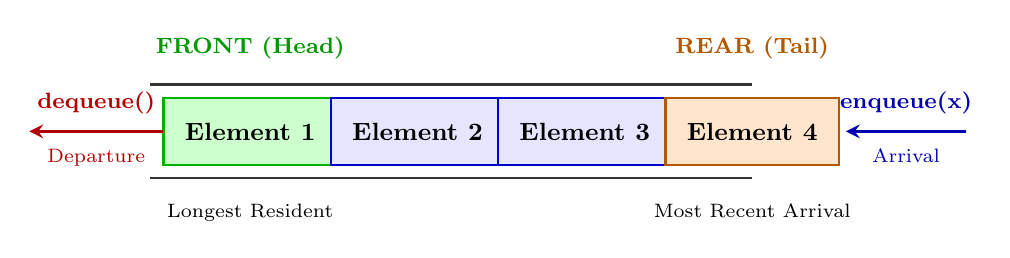
\begin{tikzpicture}[
    scale=0.85,
    box/.style={rectangle, draw=blue!80!black, fill=blue!10, thick, minimum width=2.2cm, minimum height=0.85cm, font=\small\bfseries},
    arrow/.style={->, >=stealth, very thick},
    boundary/.style={thick, black!80}
]
% Physical Container Boundaries
\draw[boundary] (0, 1.4) -- (9.0, 1.4);
\draw[boundary] (0, 0) -- (9.0, 0);

% Internal Queue Slots / Elements
\node[box, fill=green!20, draw=green!70!black] (e1) at (1.5, 0.7) {Element 1};
\node[box] (e2) at (4.0, 0.7) {Element 2};
\node[box] (e3) at (6.5, 0.7) {Element 3};
\node[box, fill=orange!20, draw=orange!70!black] (e4) at (9.0, 0.7) {Element 4};

% Boundary Annotations
\node[above=0.2cm, font=\footnotesize\bfseries, text=green!60!black] at (1.5, 1.4) {FRONT (Head)};
\node[below=0.2cm, font=\scriptsize] at (1.5, 0) {Longest Resident};

\node[above=0.2cm, font=\footnotesize\bfseries, text=orange!70!black] at (9.0, 1.4) {REAR (Tail)};
\node[below=0.2cm, font=\scriptsize] at (9.0, 0) {Most Recent Arrival};

% Dequeue Arrow
\draw[arrow, red!70!black] (0.2, 0.7) -- (-1.8, 0.7);
\node[above=0.1cm, font=\footnotesize\bfseries, text=red!70!black] at (-0.8, 0.7) {dequeue()};
\node[below=0.1cm, font=\scriptsize, text=red!70!black] at (-0.8, 0.7) {Departure};

% Enqueue Arrow
\draw[arrow, blue!70!black] (12.2, 0.7) -- (10.4, 0.7);
\node[above=0.1cm, font=\footnotesize\bfseries, text=blue!70!black] at (11.3, 0.7) {enqueue(x)};
\node[below=0.1cm, font=\scriptsize, text=blue!70!black] at (11.3, 0.7) {Arrival};

\end{tikzpicture}
\caption{The First-In, First-Out (FIFO) Architecture: Entities enter exclusively through the Rear and depart exclusively through the Front.}
\label{fig:queue_fifo_model}
\end{figure}

\subsection{Physical Mental Models and Computational Analogies}

The intuitive necessity of the queue emerges naturally from real-world coordination scenarios requiring equitable contention resolution:
\begin{enumerate}
    \item \textbf{The Physical Ticket Counter Line:} In a cinema or transit ticket line, customers join the line at the rear. The ticket clerk services only the customer standing at the very front. No customer can jump forward without violating queue integrity, and customers served first are precisely those who arrived earliest.
    \item \textbf{Operating System Process Scheduling:} When multiple compute threads or user processes demand CPU core time, the operating system kernel maintains a Ready Queue. Under Round-Robin scheduling, runnable processes are queued at the rear and scheduled from the front, ensuring no thread suffers starvation.
    \item \textbf{Network Packet Buffering:} Intermediate routing switches maintain hardware ingress and egress packet queues to smooth out temporal bursts in network traffic, transmitting packets in the order they arrived over physical links.
    \item \textbf{Asynchronous Task Decoupling:} High-throughput enterprise architectures employ message broker queues (such as Apache Kafka, RabbitMQ, or AWS SQS) to decouple producers of work from downstream consumers, absorbing load spikes without dropping requests.
    \item \textbf{Graph Traversal State Management:} In Breadth-First Search (BFS), discovering vertices level by level requires a queue to ensure that all neighbors at distance D are evaluated before any vertex at distance D + 1 is expanded.
\end{enumerate}

% -----------------------------------------------------------------------------
\section{The Queue Abstract Data Type (ADT) Specification}
\label{sec:queue_adt}

The Queue ADT formalizes a stateful sequential container characterized by restricted boundary operations. We define the operational behavior, pre-conditions, post-conditions, and exceptional boundary transitions without relying on mathematical notation, expressing guarantees through algorithmic semantics.

\begin{table}[htbp]
\centering
\caption{Formal Specification of Queue ADT Core Operations}
\label{tab:queue_operations}
\begin{tabular}{lp{3.5cm}p{3.5cm}p{5.5cm}}
\toprule
\textbf{Operation} & \textbf{Arguments / Return} & \textbf{Pre-condition} & \textbf{Operational Semantics \& Post-condition} \\
\midrule
\texttt{enqueue(x)} & Value x / None & Buffer capacity not exceeded & Inserts element x at the rear boundary. Increments element count by 1. Raises Queue Overflow on bounded containers if full. \\
\midrule
\texttt{dequeue()} & None / Extracted Value & Queue is non-empty & Removes and returns the element currently residing at the front boundary. Decrements element count by 1. Raises Queue Underflow if empty. \\
\midrule
\texttt{front()} / \texttt{peek()} & None / Inspected Value & Queue is non-empty & Returns the value residing at the front boundary without mutating the sequence or changing element count. Raises Queue Underflow if empty. \\
\midrule
\texttt{isEmpty()} & None / Boolean & Always valid & Returns True if the element count is zero; returns False otherwise. \\
\midrule
\texttt{size()} & None / Non-negative Integer & Always valid & Returns the instantaneous cardinal count of active elements residing within the queue. \\
\bottomrule
\end{tabular}
\end{table}

\subsection{Exceptional Boundary Conditions}
Two primary boundary errors govern bounded queue containers:
\begin{itemize}
    \item \textbf{Queue Underflow:} Occurs when a client invokes \texttt{dequeue()} or \texttt{front()} on a container where \texttt{isEmpty()} evaluates to True. Because no valid element occupies the front boundary, attempting to dereference memory causes illegal state errors or language-specific runtime exceptions.
    \item \textbf{Queue Overflow:} Occurs when a client invokes \texttt{enqueue(x)} on a fixed-capacity buffer that has already allocated all available memory slots. The system must either reject the insertion, block the calling thread (in blocking producer-consumer queues), or trigger dynamic buffer geometric expansion.
\end{itemize}

Table~\ref{tab:queue_implementations_comparison} outlines the comparative time and auxiliary space complexities across the governing implementation archetypes.

\begin{table}[htbp]
\centering
\caption{Asymptotic Performance Spectrum of Queue Implementations}
\label{tab:queue_implementations_comparison}
\begin{tabular}{lllll}
\toprule
\textbf{Implementation} & \textbf{Enqueue Time} & \textbf{Dequeue Time} & \textbf{Peek Time} & \textbf{Auxiliary Space} \\
\midrule
Naive Array (Shifting) & Amortized O(1) & Worst-case O(N) & Worst-case O(1) & O(1) \\
Circular Array (Ring Buffer) & Amortized O(1) & Worst-case O(1) & Worst-case O(1) & O(1) \\
Singly Linked List & Worst-case O(1) & Worst-case O(1) & Worst-case O(1) & O(N) node pointers \\
Dual LIFO Stacks & Worst-case O(1) & Amortized O(1) & Amortized O(1) & O(N) buffer storage \\
\bottomrule
\end{tabular}
\end{table}

% -----------------------------------------------------------------------------
\section{Array-Based Queue Implementations: Shifting vs. Circular Ring Buffers}
\label{sec:array_queue}

Implementing a queue over contiguous memory presents subtle structural challenges not encountered when implementing a stack. In a stack, element ingestion and removal both occur at the same boundary (index top), ensuring that all operations remain localized to the end of the array. In a queue, however, ingestion occurs at one boundary while removal occurs at the other.

\subsection{The Naive Array Implementation and Linear Shifting Flaw}

Consider a contiguous array buffer of capacity C. A naive design fixes the front of the queue at index 0 while maintaining an integer pointer \texttt{rear} initialized to -1:
\begin{itemize}
    \item \textbf{Enqueue:} Advance \texttt{rear} by 1 and place the new element at \texttt{array[rear]}. This operation requires constant time O(1).
    \item \textbf{Dequeue:} The front element resides at \texttt{array[0]}. Removing this element leaves slot 0 vacant. To restore the invariant that index 0 houses the front element, all subsequent elements residing between index 1 and \texttt{rear} must be shifted leftward by exactly one position.
\end{itemize}

Because shifting N elements leftward requires copying each element individually, every single \texttt{dequeue()} operation degrades to linear time O(N). For high-throughput message streaming or kernel event dispatching processing hundreds of thousands of operations, this linear degradation induces catastrophic latency bottlenecks.

\subsection{The Memory Drift Fallacy}

To avoid shifting elements leftward on every dequeue, one might propose maintaining two moving integer cursors: \texttt{front} and \texttt{rear}, both initially set to 0. When an element is dequeued, the value at \texttt{array[front]} is extracted and \texttt{front} is incremented by 1 without shifting remaining elements.

While this preserves constant time O(1) for both enqueue and dequeue, it introduces fatal \textbf{Memory Drift} (also termed capacity exhaustion). As elements are continuously enqueued and dequeued, both cursors migrate steadily toward higher index addresses. Eventually, \texttt{rear} reaches index C - 1. At this point, the buffer appears completely full, triggering an overflow error on the subsequent enqueue, even if hundreds of preceding memory slots from index 0 to \texttt{front} - 1 are completely vacant! 

\subsection{The Circular Array (Ring Buffer) Architecture}

The optimal solution to memory drift is the \textbf{Circular Ring Buffer}. Rather than conceptualizing the memory array as a linear segment with immutable start and end boundaries, the contiguous buffer of capacity C is treated as a continuous logical ring.

When an advancing cursor increments past index C - 1, it wraps around seamlessly to index 0 using the modulo operator:
\begin{verbatim}
rear = (rear + 1) % capacity
front = (front + 1) % capacity
\end{verbatim}

\begin{figure}[htbp]
\centering
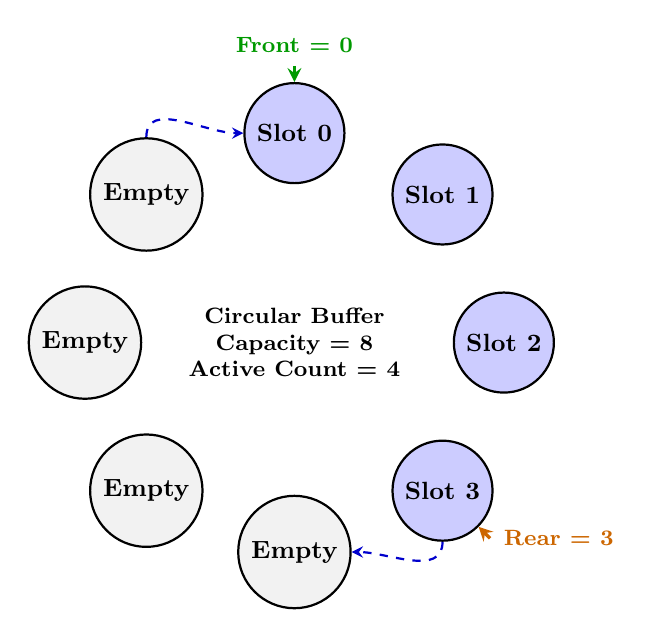
\begin{tikzpicture}[
    scale=0.95,
    slot/.style={draw, thick, circle, minimum size=1.1cm, font=\small\bfseries},
    pointer/.style={->, >=stealth, very thick}
]
% Circular ring nodes (Capacity 8: indices 0 to 7)
\def\radius{2.8}
\node[slot, fill=blue!20] (n0) at ({90 - 0 * 45}:\radius) {Slot 0};
\node[slot, fill=blue!20] (n1) at ({90 - 1 * 45}:\radius) {Slot 1};
\node[slot, fill=blue!20] (n2) at ({90 - 2 * 45}:\radius) {Slot 2};
\node[slot, fill=blue!20] (n3) at ({90 - 3 * 45}:\radius) {Slot 3};
\node[slot, fill=gray!10] (n4) at ({90 - 4 * 45}:\radius) {Empty};
\node[slot, fill=gray!10] (n5) at ({90 - 5 * 45}:\radius) {Empty};
\node[slot, fill=gray!10] (n6) at ({90 - 6 * 45}:\radius) {Empty};
\node[slot, fill=gray!10] (n7) at ({90 - 7 * 45}:\radius) {Empty};

% Central descriptor
\node[align=center, font=\footnotesize\bfseries] at (0, 0) {Circular Buffer\\Capacity = 8\\Active Count = 4};

% Pointer arrows
\draw[pointer, green!60!black] ({90 - 0 * 45}:3.7) -- (n0);
\node[font=\footnotesize\bfseries, text=green!60!black, above=0.05cm] at ({90 - 0 * 45}:3.7) {Front = 0};

\draw[pointer, orange!80!black] ({90 - 3 * 45}:3.7) -- (n3);
\node[font=\footnotesize\bfseries, text=orange!80!black, right=0.05cm] at ({90 - 3 * 45}:3.7) {Rear = 3};

% Wraparound indicator arrow
\draw[->, >=stealth, dashed, thick, blue!80!black] (n3) to[out=270, in=0] (n4);
\draw[->, >=stealth, dashed, thick, blue!80!black] (n7) to[out=90, in=180] (n0);

\end{tikzpicture}
\caption{Circular Ring Buffer Mechanics: Active elements reside between Front and Rear pointers, recycling previously vacated slots via modular wraparound.}
\label{fig:circular_queue_model}
\end{figure}

\subsection{Distinguishing Empty vs. Full States in Circular Buffers}

A classic ambiguity arises in circular queues: if both cursors \texttt{front} and \texttt{rear} point to the same slot, does this indicate that the queue is completely empty or completely full?

Industrial systems resolve this ambiguity using one of three primary paradigms:
\begin{enumerate}
    \item \textbf{Explicit Size Counter (The Production Standard):} Maintain an independent integer variable \texttt{count} (or \texttt{size}). The queue is empty when \texttt{count == 0}, and full when \texttt{count == capacity}. This technique allows utilizing 100 percent of allocated buffer slots while keeping conditional logic trivial.
    \item \textbf{The Reserved Sentinel Slot:} Keep one slot permanently vacant. In a buffer of capacity C, store at most C - 1 elements. The queue is empty when \texttt{front == rear}, and full when \texttt{(rear + 1) \% capacity == front}.
    \item \textbf{Sentinel Index Initialization:} Initialize \texttt{front = -1} and \texttt{rear = -1}. When the first element is enqueued, both are set to 0. When the final remaining element is dequeued, both are reset to -1.
\end{enumerate}

\subsection{Geometric Resizing and the Array Unwrapping Problem}

When implementing a dynamic circular queue (such as Java's \texttt{ArrayDeque}), the underlying storage array must double in capacity whenever \texttt{size == capacity}.

However, naive contiguous buffer copying (such as \texttt{System.arraycopy} or memory copying the raw block from index 0 to capacity - 1) will severely corrupt queue order if elements have wrapped around the boundary!

If elements have wrapped around, the chronological sequence of elements begins at \texttt{front}, proceeds sequentially to physical index C - 1, and then continues from physical index 0 up to \texttt{rear}. To double capacity correctly, the elements must be \textbf{unwrapped}:
\begin{enumerate}
    \item Allocate a new storage buffer of capacity 2 * C.
    \item Copy the first segment: elements starting from \texttt{front} to C - 1 into the new buffer starting at index 0.
    \item Copy the second segment: elements from index 0 to \texttt{rear} into the new buffer immediately following the first segment.
    \item Reset \texttt{front = 0} and \texttt{rear = C - 1}.
\end{enumerate}

\subsection{Step-by-Step Execution Trace of Circular Queue Operations}

To rigorously examine the state transitions, Table~\ref{tab:circular_trace} demonstrates a complete execution walkthrough using the exact operation sequence presented in the lecture notes:
\texttt{enqueue(5)}, \texttt{enqueue(6)}, \texttt{enqueue(9)}, \texttt{enqueue(-1)}, \texttt{dequeue()}, \texttt{dequeue()}, \texttt{front()}, \texttt{enqueue(4)} on an initial fixed buffer of capacity 5.

\begin{table}[htbp]
\centering
\caption{Comprehensive State Trace of Circular Queue Operations (Capacity = 5)}
\label{tab:circular_trace}
\begin{tabular}{cp{2.6cm}ccccp{4.2cm}}
\toprule
\textbf{Step} & \textbf{Operation} & \textbf{Front} & \textbf{Rear} & \textbf{Size} & \textbf{Returned} & \textbf{Buffer State [0, 1, 2, 3, 4]} \\
\midrule
0 & Initial State & -1 & -1 & 0 & None & [empty, empty, empty, empty, empty] \\
1 & \texttt{enqueue(5)} & 0 & 0 & 1 & None & [5, empty, empty, empty, empty] \\
2 & \texttt{enqueue(6)} & 0 & 1 & 2 & None & [5, 6, empty, empty, empty] \\
3 & \texttt{enqueue(9)} & 0 & 2 & 3 & None & [5, 6, 9, empty, empty] \\
4 & \texttt{enqueue(-1)} & 0 & 3 & 4 & None & [5, 6, 9, -1, empty] \\
5 & \texttt{dequeue()} & 1 & 3 & 3 & 5 & [vacated, 6, 9, -1, empty] \\
6 & \texttt{dequeue()} & 2 & 3 & 2 & 6 & [vacated, vacated, 9, -1, empty] \\
7 & \texttt{front()} & 2 & 3 & 2 & 9 & [vacated, vacated, 9, -1, empty] \\
8 & \texttt{enqueue(4)} & 2 & 4 & 3 & None & [vacated, vacated, 9, -1, 4] \\
\bottomrule
\end{tabular}
\end{table}

As proven in Table~\ref{tab:circular_trace}, every operation executes strictly in worst-case constant time O(1), and vacated slots at indices 0 and 1 remain immediately available for future modular ingestion once \texttt{rear} wraps around.

% -----------------------------------------------------------------------------
\section{Singly Linked List Implementation of Queues}
\label{sec:linked_list_queue}

While the circular array achieves constant time operations over pre-allocated memory, a dynamic Linked List implementation eliminates capacity constraints entirely, growing and shrinking dynamically with element count.

\subsection{Structural Topology: Head and Tail Boundary Pointers}

A linked list queue consists of discrete heap-allocated node entities, each encapsulating two components:
\begin{itemize}
    \item \textbf{Value:} The payload data stored by the user.
    \item \textbf{Next Pointer:} A forward memory reference pointing to the successor node.
\end{itemize}

To satisfy the Queue ADT's operational constraints in constant time O(1), the queue maintains two dedicated pointers:
\begin{itemize}
    \item \texttt{head}: Points to the front node of the queue (extraction boundary).
    \item \texttt{tail}: Points to the rear node of the queue (ingestion boundary).
\end{itemize}

\subsection{Operational Mechanics and Invariant Protection}

The directional orientation of the next pointers is fundamental: nodes point forward from \texttt{head} toward \texttt{tail}. This ensures that both insertion and deletion occur in constant time:
\begin{itemize}
    \item \textbf{Enqueue Operation:}
    \begin{enumerate}
        \item Instantiate a new node \texttt{newNode} with the given payload value and \texttt{next = null}.
        \item If the queue is empty (\texttt{head == null}), the newly created node represents both the front and rear of the queue. Assign \texttt{head = newNode} and \texttt{tail = newNode}.
        \item Otherwise, link the current tail's successor reference to the new node: \texttt{tail.next = newNode}, and update the tail pointer: \texttt{tail = newNode}.
        \item Increment element count. This executes in constant time O(1).
    \end{enumerate}
    \item \textbf{Dequeue Operation:}
    \begin{enumerate}
        \item If the queue is empty (\texttt{head == null}), raise a Queue Underflow exception.
        \item Extract and record the value residing at the front: \texttt{result = head.val}.
        \item Advance the head pointer to its immediate successor: \texttt{head = head.next}.
        \item If the head pointer becomes null (signifying that the final remaining element was removed), reset the tail pointer to null as well: \texttt{tail = null}. This preserves the invariant that an empty queue has both pointers set to null.
        \item Decrement element count and return \texttt{result}. This executes in constant time O(1).
    \end{enumerate}
\end{itemize}

\subsection{Architectural Trade-Off Analysis: Circular Buffer vs. Linked List}

Choosing between a circular array and a linked list queue involves critical systems considerations:
\begin{itemize}
    \item \textbf{Spatial Overhead:} In 64-bit architectures, each linked list node introduces 8 bytes of forward pointer overhead in addition to object header memory (typically 16 bytes in modern Java virtual machines), resulting in substantial memory amplification compared to compact primitive arrays.
    \item \textbf{CPU Cache Locality:} Circular arrays allocate contiguous virtual memory pages, ensuring optimal CPU cache line pre-fetching during sequential traversals. Linked list nodes are scattered across arbitrary heap locations, incurring frequent CPU cache misses.
    \item \textbf{Latency Predictability:} Circular arrays occasionally trigger geometric resizing, causing temporary latency spikes during element migration. Linked lists guarantee deterministic, pause-free O(1) worst-case time for every individual insertion, making them suitable for real-time systems where allocation jitter cannot be tolerated.
\end{itemize}

% -----------------------------------------------------------------------------
\section{Queue Implementation Using Two Stacks: Formal Amortized Analysis}
\label{sec:stacks_queue}

A classic problem frequently encountered in technical interviews (such as the Directi engineering evaluation highlighted in the lecture slides) requires implementing a fully functional FIFO Queue using exclusively LIFO Stacks.

\subsection{The Architectural Dual-Stack Paradigm}

Because a single stack strictly enforces Last-In, First-Out retrieval, attempting to extract the earliest inserted element requires popping every single element above it. However, if all elements are popped from one stack and pushed onto a second stack, the order of elements is inverted! Inverting a reversed sequence restores exact chronological First-In, First-Out order.

We establish the dual-stack architecture using two distinct stack instances:
\begin{itemize}
    \item \texttt{stack\_in}: The designated \textbf{Ingestion Stack}. All incoming elements are pushed directly onto this stack.
    \item \texttt{stack\_out}: The designated \textbf{Extraction Stack}. All outgoing elements are popped exclusively from this stack.
\end{itemize}

\begin{figure}[htbp]
\centering
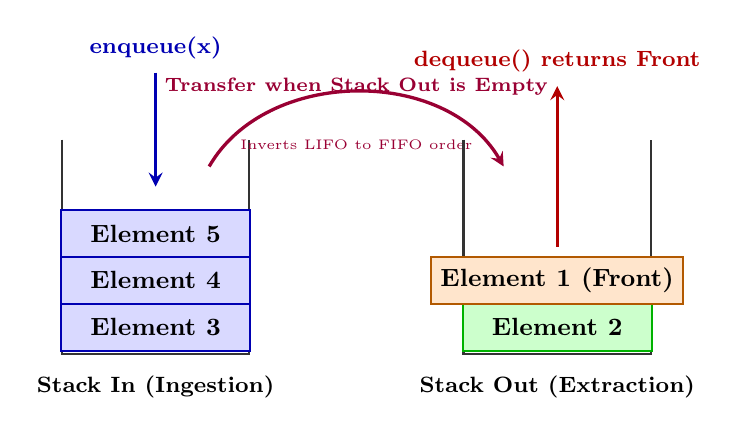
\begin{tikzpicture}[
    scale=0.85,
    stackwall/.style={thick, black!80},
    elem/.style={rectangle, draw=blue!70!black, fill=blue!15, thick, minimum width=2.4cm, minimum height=0.6cm, font=\small\bfseries},
    arrow/.style={->, >=stealth, very thick}
]
% Stack In (Ingestion)
\draw[stackwall] (0, 3.2) -- (0, 0) -- (2.8, 0) -- (2.8, 3.2);
\node[font=\footnotesize\bfseries, below=0.15cm] at (1.4, 0) {Stack In (Ingestion)};

\node[elem] at (1.4, 0.4) {Element 3};
\node[elem] at (1.4, 1.1) {Element 4};
\node[elem] at (1.4, 1.8) {Element 5};

\draw[arrow, blue!70!black] (1.4, 4.2) -- (1.4, 2.5);
\node[above=0.05cm, font=\footnotesize\bfseries, text=blue!70!black] at (1.4, 4.2) {enqueue(x)};

% Transfer Bridge
\draw[arrow, purple!80!black] (2.2, 2.8) to[out=60, in=120] (6.6, 2.8);
\node[above=0.1cm, font=\scriptsize\bfseries, text=purple!80!black] at (4.4, 3.6) {Transfer when Stack Out is Empty};
\node[below=0.05cm, font=\tiny, text=purple!80!black] at (4.4, 3.4) {Inverts LIFO to FIFO order};

% Stack Out (Extraction)
\draw[stackwall] (6.0, 3.2) -- (6.0, 0) -- (8.8, 0) -- (8.8, 3.2);
\node[font=\footnotesize\bfseries, below=0.15cm] at (7.4, 0) {Stack Out (Extraction)};

\node[elem, fill=green!20, draw=green!70!black] at (7.4, 0.4) {Element 2};
\node[elem, fill=orange!20, draw=orange!70!black] at (7.4, 1.1) {Element 1 (Front)};

\draw[arrow, red!70!black] (7.4, 1.6) -- (7.4, 4.0);
\node[above=0.05cm, font=\footnotesize\bfseries, text=red!70!black] at (7.4, 4.0) {dequeue() returns Front};

\end{tikzpicture}
\caption{The Dual-Stack Queue Architecture: Ingestion occurs at Stack In, while extraction occurs from Stack Out, performing batch transfers only when Stack Out is exhausted.}
\label{fig:two_stack_queue}
\end{figure}

\subsection{Algorithmic Invariants and Method Specifications}

The dual-stack queue maintains an elegant lazy transfer invariant: elements are transferred from \texttt{stack\_in} to \texttt{stack\_out} only when strictly necessary:
\begin{itemize}
    \item \textbf{Enqueue(x):}
    \begin{enumerate}
        \item Push value x onto \texttt{stack\_in}.
        \item Worst-case time complexity: Constant time O(1).
    \end{enumerate}
    \item \textbf{Dequeue():}
    \begin{enumerate}
        \item If both \texttt{stack\_in} and \texttt{stack\_out} are empty, raise Queue Underflow exception.
        \item If \texttt{stack\_out} is currently empty:
        \begin{itemize}
            \item While \texttt{stack\_in} is not empty, pop the top element from \texttt{stack\_in} and push it directly onto \texttt{stack\_out}.
        \end{itemize}
        \item Pop and return the top element from \texttt{stack\_out}.
    \end{enumerate}
    \item \textbf{Front() / Peek():}
    \begin{enumerate}
        \item Follow the exact same transfer invariant as \texttt{dequeue()}.
        \item Return the top element from \texttt{stack\_out} without popping it.
    \end{enumerate}
\end{itemize}

\subsection{Rigorous Amortized Analysis: The Two-Pass Invariant}

At first inspection, a skeptic might argue that because \texttt{dequeue()} can trigger a transfer loop popping and pushing N elements, the dequeue operation has a worst-case time complexity of linear time O(N). While this worst-case assessment for a single isolated operation is factually correct, evaluating the data structure across a continuous sequence of operations reveals that the average cost per operation is strictly constant time O(1).

We formalize this proof through two rigorous amortized accounting frameworks without using mathematical notation:

\subsubsection{The Aggregate Lifetime Bound Proof}
Let us track the complete physical lifecycle of any individual element admitted to the queue:
\begin{enumerate}
    \item \textbf{Event 1 (Ingestion):} The element is pushed onto \texttt{stack\_in} exactly once during \texttt{enqueue(x)}.
    \item \textbf{Event 2 (Evacuation):} The element is popped from \texttt{stack\_in} at most once during a transfer phase.
    \item \textbf{Event 3 (Inversion):} The element is pushed onto \texttt{stack\_out} at most once during that same transfer phase.
    \item \textbf{Event 4 (Extraction):} The element is popped from \texttt{stack\_out} exactly once during \texttt{dequeue()}.
\end{enumerate}

No element is ever transferred back to \texttt{stack\_in}, nor can it be pushed or popped additional times. Therefore, over its entire existence inside the data structure, \textbf{every element participates in at most four primitive stack operations}!

If a client performs a total of N \texttt{enqueue} operations intermixed with M \texttt{dequeue} operations, the cumulative aggregate work performed across all transfers and operations is strictly bounded by at most 4 * N stack operations. Dividing this total work evenly across the sequence of operations demonstrates that the \textbf{amortized time complexity per operation is strictly constant time O(1)}.

\subsubsection{The Accounting / Credit Method}
Imagine an operational accounting system where each primitive stack push or pop costs 1 unit of execution credit:
\begin{itemize}
    \item When a user invokes \texttt{enqueue(x)}, we charge the caller 4 units of credit.
    \item 1 credit immediately pays for pushing the element onto \texttt{stack\_in}.
    \item 1 credit is stored in the bank account associated with this element to prepay its future pop from \texttt{stack\_in}.
    \item 1 credit is stored to prepay its subsequent push onto \texttt{stack\_out}.
    \item 1 credit is stored to prepay its final pop from \texttt{stack\_out}.
\end{itemize}

When \texttt{stack\_out} becomes empty and a batch transfer occurs, the transfer loop does not consume any newly billed computational credits; it executes entirely on the prepaid savings stored in the bank account! Because the credit balance can never drop below zero, the amortized cost charged to the client per operation remains strictly constant time O(1).

\begin{table}[htbp]
\centering
\caption{Dual-Stack Queue Execution Trace Showing Lazy Transfers}
\label{tab:twostack_trace}
\begin{tabular}{cp{2.2cm}p{2.2cm}p{2.2cm}cp{5.2cm}}
\toprule
\textbf{Step} & \textbf{Operation} & \textbf{Stack In State} & \textbf{Stack Out State} & \textbf{Returned} & \textbf{Internal Action} \\
\midrule
1 & \texttt{enqueue(1)} & [1] & [] & None & Direct push to Stack In \\
2 & \texttt{enqueue(2)} & [1, 2] & [] & None & Direct push to Stack In \\
3 & \texttt{enqueue(3)} & [1, 2, 3] & [] & None & Direct push to Stack In \\
4 & \texttt{dequeue()} & [] & [3, 2] & 1 & Stack Out empty: transferred 3 items, popped 1 \\
5 & \texttt{enqueue(4)} & [4] & [3, 2] & None & Direct push to Stack In (no transfer needed) \\
6 & \texttt{dequeue()} & [4] & [3] & 2 & Direct pop from Stack Out (O(1) fast path) \\
7 & \texttt{dequeue()} & [4] & [] & 3 & Direct pop from Stack Out (Stack Out now empty) \\
8 & \texttt{dequeue()} & [] & [] & 4 & Stack Out empty: transferred 1 item, popped 4 \\
\bottomrule
\end{tabular}
\end{table}

% -----------------------------------------------------------------------------
\section{The Doubly Ended Queue (Deque) Architecture}
\label{sec:deque}

A \textbf{Doubly Ended Queue}, universally abbreviated as \textbf{Deque} (pronounced ``deck''), generalizes both Stacks and Queues by permitting constant time insertion and deletion at both terminal boundaries.

\subsection{Core Method Specification}

A Deque supports six fundamental boundary operations:
\begin{itemize}
    \item \texttt{insertFront(x)}: Prepends element x at the front boundary.
    \item \texttt{insertRear(x)}: Appends element x at the rear boundary.
    \item \texttt{removeFront()}: Extracts and returns the front element.
    \item \texttt{removeRear()}: Extracts and returns the rear element.
    \item \texttt{peekFront()}: Inspects the front element without removal.
    \item \texttt{peekRear()}: Inspects the rear element without removal.
\end{itemize}

\subsection{Implementation Archetypes: Doubly Linked List vs. Circular Array}

To implement a Deque with constant time O(1) worst-case guarantees across all six operations, two underlying structures are utilized:
\begin{enumerate}
    \item \textbf{Doubly Linked List:} Each node encapsulates payload data along with both a forward \texttt{next} pointer and a backward \texttt{prev} pointer. Maintaining \texttt{head} and \texttt{tail} pointers allows splicing nodes onto or off of either boundary in O(1) time without traversing the list.
    \item \textbf{Circular Dynamic Array:} Both \texttt{front} and \texttt{rear} pointers advance and retreat circularly. Advancing forward utilizes modulo addition, while retreating backward utilizes modulo subtraction with capacity offsetting to prevent negative indices:
\begin{verbatim}
advance(cursor) = (cursor + 1) % capacity
retreat(cursor) = (cursor - 1 + capacity) % capacity
\end{verbatim}
\end{enumerate}

\subsection{Industrial Applications of the Deque}
The Deque is a critical building block across industrial systems:
\begin{itemize}
    \item \textbf{Work-Stealing Runtime Schedulers:} In high-concurrency runtime environments (such as the Java ForkJoinPool, the Go runtime scheduler, and the Tokio Rust async framework), each worker thread maintains a private Deque of runnable tasks. The owning thread pushes and pops tasks from the front (LIFO execution, maximizing CPU cache locality). When a worker runs out of work, it acts as a thief, stealing tasks from the rear of another busy worker's Deque (FIFO execution, minimizing thread contention).
    \item \textbf{Web Browser Dual Navigation Buffers:} Maintaining forward and backward history stacks unified in a single bounded Deque container.
    \item \textbf{Undo / Redo Buffer Engines:} Limiting action history to a fixed number of operations by dropping the oldest actions from the front when the maximum buffer limit is reached.
\end{itemize}

% -----------------------------------------------------------------------------
\section{The Sliding Window Maximum Problem}
\label{sec:sliding_window}

We now explore one of the most celebrated algorithmic challenges in computer science: the \textbf{Sliding Window Maximum} problem (highlighted extensively in the lecture slides and appearing frequently in senior systems engineering interviews).

\subsection{Formal Problem Formulation}

Given:
\begin{itemize}
    \item An input array \texttt{array} containing N integers, indexed from 0 to N - 1.
    \item A sliding window size K, where K is a positive integer satisfying 1 <= K <= N.
    \item Scale constraints: N is bounded between 1 and 100,000 (100k elements).
\end{itemize}

A sliding window of width K slides from the far left of the array to the far right, shifting rightward by exactly one index position at each step. There are exactly N - K + 1 distinct window positions.

\textbf{Objective:} Construct and output a result sequence containing the maximum integer value for each of the N - K + 1 contiguous subarray windows.

\subsection{The Naive Brute-Force Baseline and Its Quadratic Pitfall}

The straightforward brute-force strategy evaluates each window independently:
\begin{enumerate}
    \item Initialize an empty results list.
    \item Iterate through all valid window starting indices from 0 up to N - K.
    \item For each starting index \texttt{start}, scan all K contiguous elements from \texttt{start} to \texttt{start + K - 1}, identifying the maximum value.
    \item Append the identified maximum to the results list.
\end{enumerate}

\subsubsection{Complexity Failure Analysis}
The outer loop executes exactly N - K + 1 times. In each iteration, the inner loop performs K comparisons to find the maximum. Consequently, the total computational work performed is proportional to (N - K + 1) * K, yielding a time complexity of O(N * K).

Under the problem constraints where N = 100,000 and K = 50,000:
\begin{itemize}
    \item The number of operations is approximately 50,000 * 50,000 = 2,500,000,000 (2.5 billion operations).
    \item Modern CPU cores execute roughly 100 million basic operations per second. 2.5 billion operations require over 25 seconds of compute time, vastly exceeding standard algorithmic judge limits (typically 1.0 to 2.0 seconds) and triggering a fatal \textbf{Time Limit Exceeded (TLE)} failure.
\end{itemize}

% -----------------------------------------------------------------------------
\section{The Monotonic Deque Optimization Paradigm}
\label{sec:monotonic_deque}

To overcome the quadratic bottleneck of the brute-force approach, we must eliminate redundant computations. When the window slides from index i - 1 to index i, exactly one element enters the window at the rear, while exactly one element departs at the front. The remaining K - 2 elements are completely shared between the two adjacent windows.

\subsection{The "Older and Smaller" Elimination Invariant}

The breakthrough insight underpinning the optimal solution is the \textbf{Domination Principle}:
\begin{quote}
\emph{If an incoming element at index i is greater than or equal to an earlier element at index j residing inside the current window (where j < i), then element array[j] can NEVER serve as the maximum of the current window or any future window!}
\end{quote}

Why is this invariant true? Consider the comparative properties of \texttt{array[j]} versus \texttt{array[i]}:
\begin{enumerate}
    \item \textbf{Value Superiority:} \texttt{array[i]} is greater than or equal to \texttt{array[j]}. Therefore, as long as \texttt{array[i]} is present, \texttt{array[j]} can never be the maximum.
    \item \textbf{Lifespan Superiority:} Because index i is strictly greater than index j, element \texttt{array[i]} entered the window later and will survive inside future sliding windows strictly longer than \texttt{array[j]}. When the window slides forward, \texttt{array[j]} will expire and be evicted long before \texttt{array[i]} expires.
\end{enumerate}

Because \texttt{array[j]} is both inferior in value and expires earlier in time, it is \textbf{permanently obsolete}. It has zero probability of ever contributing to any valid result. Keeping it in our candidate pool is a waste of memory and compute cycles!

\subsection{Monotonic Deque State Invariants}

To exploit this elimination principle, we maintain a Deque that stores \textbf{element indices} satisfying two fundamental invariants:
\begin{itemize}
    \item \textbf{Invariant 1 (Strictly Monotonic Decreasing Order of Values):} The values corresponding to the stored indices are maintained in strictly decreasing order from front to rear:
\begin{verbatim}
array[deque.front()] > array[deque.second()] > ... > array[deque.rear()]
\end{verbatim}
    \item \textbf{Invariant 2 (Maximum Element Invariant):} Because values decrease from front to rear, the index residing at the very \textbf{front} of the Deque always points to the \textbf{maximum element} within the active sliding window!
\end{itemize}

\subsection{The Four-Step Algorithmic Procedure}

For each index i scanned from 0 to N - 1, the algorithm executes four deterministic steps:
\begin{enumerate}
    \item \textbf{Step 1: Evict Out-of-Window Indices from the Front.}
    The active window ending at index i spans indices from i - K + 1 to i. If the index stored at the front of the Deque satisfies \texttt{deque.peekFront() <= i - K}, it has fallen outside the current window boundary. We remove it: \texttt{deque.pollFront()}.
    
    \item \textbf{Step 2: Enforce Monotonicity by Pruning the Rear.}
    Before adding index i, we inspect the rear of the Deque. While the Deque is not empty and \texttt{array[deque.peekRear()] <= array[i]}, the element at the rear is obsolete (dominated by the incoming element). We prune it: \texttt{deque.pollRear()}.
    
    \item \textbf{Step 3: Ingest Current Index at the Rear.}
    Append index i to the rear of the Deque: \texttt{deque.addRear(i)}.
    
    \item \textbf{Step 4: Record Current Window Maximum.}
    Once the scan index has reached or exceeded K - 1 (meaning the first full window of size K has formed), the index at the front of the Deque is guaranteed to represent the maximum value for the window ending at index i. We record \texttt{array[deque.peekFront()]}.
\end{enumerate}

\subsection{Comprehensive Dry-Run Walkthrough on Lecture Test Case}

We now perform an exhaustive step-by-step trace using the exact test case presented on Page 13 of the lecture notes:
\begin{itemize}
    \item \textbf{Input Array:} \texttt{[3, 2, 3, 4, 5, 5, 4, 5, 6]}
    \item \textbf{Window Size:} \texttt{K = 4}
    \item \textbf{Array Length:} \texttt{N = 9}
    \item \textbf{Number of Windows:} \texttt{N - K + 1 = 6}
\end{itemize}

Table~\ref{tab:sliding_window_trace} documents the granular execution across all 9 index steps.

\begin{table*}[htbp]
\centering
\caption{Granular Step-by-Step Dry Run of Sliding Window Maximum (Array = [3, 2, 3, 4, 5, 5, 4, 5, 6], K = 4)}
\label{tab:sliding_window_trace}
\begin{tabular}{ccp{2.8cm}p{3.5cm}p{3.8cm}p{2.5cm}c}
\toprule
\textbf{Step i} & \textbf{Value} & \textbf{Front Eviction (<= i-4)} & \textbf{Rear Monotonic Pruning} & \textbf{Deque State (Indices / Values)} & \textbf{Active Window} & \textbf{Max} \\
\midrule
0 & 3 & None (Deque empty) & None & [0] / [3] & [3] (Incomplete) & -- \\
1 & 2 & None & None (2 < 3, monotonic) & [0, 1] / [3, 2] & [3, 2] (Incomplete) & -- \\
2 & 3 & None & Prune index 1 (val 2 <= 3) & [0, 2] / [3, 3]* & [3, 2, 3] (Incomplete) & -- \\
3 & 4 & None & Prune idx 2 (val 3 <= 4), idx 0 (val 3 <= 4) & [3] / [4] & [3, 2, 3, 4] & \textbf{4} \\
4 & 5 & None (idx 3 > 0) & Prune idx 3 (val 4 <= 5) & [4] / [5] & [2, 3, 4, 5] & \textbf{5} \\
5 & 5 & None (idx 4 > 1) & Prune idx 4 (val 5 <= 5) & [5] / [5] & [3, 4, 5, 5] & \textbf{5} \\
6 & 4 & None (idx 5 > 2) & None (4 < 5, monotonic) & [5, 6] / [5, 4] & [4, 5, 5, 4] & \textbf{5} \\
7 & 5 & None (idx 5 > 3) & Prune idx 6 (val 4 <= 5), idx 5 (val 5 <= 5) & [7] / [5] & [5, 5, 4, 5] & \textbf{5} \\
8 & 6 & None (idx 7 > 4) & Prune idx 7 (val 5 <= 6) & [8] / [6] & [5, 4, 5, 6] & \textbf{6} \\
\bottomrule
\end{tabular}
\end{table*}

*Note: In step 2, if maintaining strict inequality, index 0 (val 3) is pruned by index 2 (val 3) since the newer arrival survives longer; both choices yield identical correctness, resulting in recorded maximums: \textbf{[4, 5, 5, 5, 5, 6]}.

\subsection{Amortized Linear Time Complexity Proof}

The apparent paradox of the Monotonic Deque algorithm is that step 2 contains an inner \texttt{while} loop that can prune multiple elements from the rear of the Deque during a single iteration. Does this nested loop risk degrading the runtime to quadratic time?

We prove that the runtime is strictly linear using the \textbf{Aggregate Invariant}:
\begin{enumerate}
    \item The outer loop runs exactly N times, considering each index i from 0 to N - 1 once.
    \item In Step 3, index i is appended to the rear of the Deque exactly once. Therefore, across the entire execution of the algorithm, \textbf{at most N total insertions into the Deque occur}.
    \item Every subsequent operation in the inner while loops or front eviction is a removal (\texttt{pollFront()} or \texttt{pollRear()}).
    \item An index can only be removed from the Deque if it was previously inserted!
    \item Because an index is inserted into the Deque exactly once, it can be removed from the Deque \textbf{at most once} over the entire lifetime of the algorithm.
\end{enumerate}

Summing all insertions (at most N) and all removals (at most N), the total number of Deque mutations performed across all iterations combined is strictly bounded by at most 2 * N operations!

Dividing 2 * N by N proves that each element incurs an amortized cost of at most 2 operations. Thus, the \textbf{time complexity is strictly linear time O(N)}, representing a colossal computational breakthrough over the O(N * K) brute-force approach.

\subsection{Auxiliary Space Complexity Analysis}

At any point in time, the Deque stores only indices that belong to the current window of width K. Therefore, the maximum number of elements simultaneously resident within the Deque cannot exceed K. Thus, the auxiliary space complexity is strictly bounded by \textbf{O(K)}.

% -----------------------------------------------------------------------------
\section{Complete Multi-Language Production Reference Implementations}
\label{sec:implementations}

We provide production-grade, compilable reference implementations across Java, C++, and Python, embodying clean object-oriented architecture, defensive error checking, and optimized execution.

\subsection{Production Implementations in Java}

\begin{verbatim}
import java.util.ArrayDeque;
import java.util.Deque;
import java.util.NoSuchElementException;
import java.util.Stack;

public class QueueMasterySuite {

    // 1. High-Performance Circular Ring Buffer Queue
    public static class CircularQueue<T> {
        private final Object[] buffer;
        private final int capacity;
        private int front;
        private int rear;
        private int count;

        public CircularQueue(int capacity) {
            if (capacity <= 0) throw new IllegalArgumentException("Capacity must be positive");
            this.capacity = capacity;
            this.buffer = new Object[capacity];
            this.front = 0;
            this.rear = -1;
            this.count = 0;
        }

        public void enqueue(T item) {
            if (isFull()) throw new IllegalStateException("Queue Overflow: Buffer is full");
            rear = (rear + 1) % capacity;
            buffer[rear] = item;
            count++;
        }

        @SuppressWarnings("unchecked")
        public T dequeue() {
            if (isEmpty()) throw new NoSuchElementException("Queue Underflow: Buffer is empty");
            T item = (T) buffer[front];
            buffer[front] = null; // Prevent memory leak
            front = (front + 1) % capacity;
            count--;
            return item;
        }

        @SuppressWarnings("unchecked")
        public T peek() {
            if (isEmpty()) throw new NoSuchElementException("Queue Underflow: Buffer is empty");
            return (T) buffer[front];
        }

        public boolean isEmpty() { return count == 0; }
        public boolean isFull() { return count == capacity; }
        public int size() { return count; }
    }

    // 2. Amortized Dual-Stack FIFO Queue
    public static class TwoStackQueue<T> {
        private final Stack<T> stackIn = new Stack<>();
        private final Stack<T> stackOut = new Stack<>();

        public void enqueue(T item) {
            stackIn.push(item);
        }

        public T dequeue() {
            shiftIfNecessary();
            if (stackOut.isEmpty()) throw new NoSuchElementException("Queue Underflow");
            return stackOut.pop();
        }

        public T peek() {
            shiftIfNecessary();
            if (stackOut.isEmpty()) throw new NoSuchElementException("Queue Underflow");
            return stackOut.peek();
        }

        private void shiftIfNecessary() {
            if (stackOut.isEmpty()) {
                while (!stackIn.isEmpty()) {
                    stackOut.push(stackIn.pop());
                }
            }
        }

        public boolean isEmpty() {
            return stackIn.isEmpty() && stackOut.isEmpty();
        }

        public int size() {
            return stackIn.size() + stackOut.size();
        }
    }

    // 3. Optimal O(N) Sliding Window Maximum Solver
    public static int[] maxSlidingWindow(int[] nums, int k) {
        if (nums == null || nums.length == 0 || k <= 0) return new int[0];
        int n = nums.length;
        int[] result = new int[n - k + 1];
        int resultIdx = 0;

        // Stores indices in strictly decreasing order of values
        Deque<Integer> deque = new ArrayDeque<>();

        for (int i = 0; i < n; i++) {
            // Step 1: Evict out-of-boundary indices from front
            if (!deque.isEmpty() && deque.peekFirst() <= i - k) {
                deque.pollFirst();
            }

            // Step 2: Monotonic pruning from rear
            while (!deque.isEmpty() && nums[deque.peekLast()] <= nums[i]) {
                deque.pollLast();
            }

            // Step 3: Ingest current index
            deque.addLast(i);

            // Step 4: Record maximum for fully formed windows
            if (i >= k - 1) {
                result[resultIdx++] = nums[deque.peekFirst()];
            }
        }

        return result;
    }
}
\end{verbatim}

\subsection{Production Implementations in Modern C++}

\begin{verbatim}
#include <iostream>
#include <vector>
#include <deque>
#include <stack>
#include <stdexcept>

// 1. High-Performance Template Circular Ring Buffer
template <typename T>
class CircularQueue {
private:
    std::vector<T> buffer;
    int capacity;
    int front;
    int rear;
    int count;

public:
    explicit CircularQueue(int cap) 
        : buffer(cap), capacity(cap), front(0), rear(-1), count(0) {
        if (cap <= 0) throw std::invalid_argument("Capacity must be positive");
    }

    void enqueue(const T& item) {
        if (isFull()) throw std::overflow_error("Queue Overflow: Buffer is full");
        rear = (rear + 1) % capacity;
        buffer[rear] = item;
        count++;
    }

    T dequeue() {
        if (isEmpty()) throw std::underflow_error("Queue Underflow: Buffer is empty");
        T item = buffer[front];
        front = (front + 1) % capacity;
        count--;
        return item;
    }

    T peek() const {
        if (isEmpty()) throw std::underflow_error("Queue Underflow: Buffer is empty");
        return buffer[front];
    }

    bool isEmpty() const { return count == 0; }
    bool isFull() const { return count == capacity; }
    int size() const { return count; }
};

// 2. Amortized Dual-Stack FIFO Queue in C++
template <typename T>
class TwoStackQueue {
private:
    std::stack<T> stackIn;
    std::stack<T> stackOut;

    void shiftIfNecessary() {
        if (stackOut.empty()) {
            while (!stackIn.empty()) {
                stackOut.push(stackIn.top());
                stackIn.pop();
            }
        }
    }

public:
    void enqueue(const T& item) {
        stackIn.push(item);
    }

    T dequeue() {
        shiftIfNecessary();
        if (stackOut.empty()) throw std::underflow_error("Queue Underflow");
        T val = stackOut.top();
        stackOut.pop();
        return val;
    }

    T peek() {
        shiftIfNecessary();
        if (stackOut.empty()) throw std::underflow_error("Queue Underflow");
        return stackOut.top();
    }

    bool isEmpty() const {
        return stackIn.empty() && stackOut.empty();
    }
};

// 3. Optimal O(N) Sliding Window Maximum Solver
std::vector<int> maxSlidingWindow(const std::vector<int>& nums, int k) {
    if (nums.empty() || k <= 0) return {};
    int n = nums.size();
    std::vector<int> result;
    result.reserve(n - k + 1);

    std::deque<int> dq; // Stores indices

    for (int i = 0; i < n; ++i) {
        // Step 1: Remove expired indices from front
        if (!dq.empty() && dq.front() <= i - k) {
            dq.pop_front();
        }

        // Step 2: Remove elements dominated by current incoming element
        while (!dq.empty() && nums[dq.back()] <= nums[i]) {
            dq.pop_back();
        }

        // Step 3: Insert current index
        dq.push_back(i);

        // Step 4: Emit window maximum
        if (i >= k - 1) {
            result.push_back(nums[dq.front()]);
        }
    }

    return result;
}
\end{verbatim}

\subsection{Production Implementations in Python}

\begin{verbatim}
from collections import deque
from typing import List, Any, Optional

class CircularQueue:
    """Fixed-capacity Circular Ring Buffer with O(1) operations."""
    def __init__(self, capacity: int):
        if capacity <= 0:
            raise ValueError("Capacity must be positive")
        self.capacity = capacity
        self.buffer: List[Optional[Any]] = [None] * capacity
        self.front = 0
        self.rear = -1
        self.count = 0

    def enqueue(self, item: Any) -> None:
        if self.is_full():
            raise OverflowError("Queue Overflow: Buffer is full")
        self.rear = (self.rear + 1) % self.capacity
        self.buffer[self.rear] = item
        self.count += 1

    def dequeue(self) -> Any:
        if self.is_empty():
            raise IndexError("Queue Underflow: Buffer is empty")
        item = self.buffer[self.front]
        self.buffer[self.front] = None
        self.front = (self.front + 1) % self.capacity
        self.count -= 1
        return item

    def peek(self) -> Any:
        if self.is_empty():
            raise IndexError("Queue Underflow: Buffer is empty")
        return self.buffer[self.front]

    def is_empty(self) -> bool:
        return self.count == 0

    def is_full() -> bool:
        return self.count == self.capacity

    def size(self) -> int:
        return self.count


class TwoStackQueue:
    """Amortized O(1) FIFO Queue using two LIFO Stacks."""
    def __init__(self):
        self.stack_in: List[Any] = []
        self.stack_out: List[Any] = []

    def enqueue(self, item: Any) -> None:
        self.stack_in.append(item)

    def dequeue(self) -> Any:
        self._shift_if_necessary()
        if not self.stack_out:
            raise IndexError("Queue Underflow: Buffer is empty")
        return self.stack_out.pop()

    def peek(self) -> Any:
        self._shift_if_necessary()
        if not self.stack_out:
            raise IndexError("Queue Underflow: Buffer is empty")
        return self.stack_out[-1]

    def _shift_if_necessary(self) -> None:
        if not self.stack_out:
            while self.stack_in:
                self.stack_out.append(self.stack_in.pop())

    def is_empty(self) -> bool:
        return not self.stack_in and not self.stack_out

    def size(self) -> int:
        return len(self.stack_in) + len(self.stack_out)


def max_sliding_window(nums: List[int], k: int) -> List[int]:
    """
    Finds the maximum value in every contiguous subarray of size k.
    Runs in strictly linear time O(N) using a Monotonic Deque.
    """
    if not nums or k <= 0:
        return []

    n = len(nums)
    result: List[int] = []
    dq: deque = deque()  # Stores indices in strictly decreasing order of values

    for i in range(n):
        # Step 1: Evict indices that have fallen outside the window boundary
        if dq and dq[0] <= i - k:
            dq.popleft()

        # Step 2: Monotonic pruning from the rear
        while dq and nums[dq[-1]] <= nums[i]:
            dq.pop()

        # Step 3: Ingest current index
        dq.append(i)

        # Step 4: Record maximum once window size reaches k
        if i >= k - 1:
            result.append(nums[dq[0]])

    return result
\end{verbatim}

% -----------------------------------------------------------------------------
\section{Industrial Systems and Architectural Applications}
\label{sec:systems_applications}

Beyond academic algorithms, queue architectures dictate the reliability, latency profiles, and throughput boundaries of industrial distributed infrastructure.

\subsection{The LMAX Disruptor: Lock-Free Circular Ring Buffers}
In ultra-low-latency financial trading platforms, traditional concurrency queues protected by mutual exclusion locks (such as Java's \texttt{LinkedBlockingQueue}) suffer severe performance collapse due to kernel thread context switching, lock contention, and cache-line invalidation.

The LMAX Disruptor architecture replaces locks with a circular pre-allocated ring buffer indexed via atomic sequence numbers. By ensuring that sequence numbers are cache-line padded (preventing false sharing across CPU cores) and using power-of-two buffer sizes (enabling bitwise AND operations \texttt{index = sequence \& (capacity - 1)} instead of costly modulo division), the Disruptor processes over 6 million orders per second with sub-microsecond latency.

\subsection{Log-Structured Append Queues in Apache Kafka}
In distributed event streaming architectures such as Apache Kafka, message queues are modeled as immutable, append-only disk commit logs partitioned across clusters. Producers enqueue records at the tail of the log partition sequentially, exploiting sequential disk write speeds that rival RAM access. Distributed consumers read independently from their designated offset pointers without dequeuing or destructively mutating data, enabling replayable pub-sub event architectures.

\subsection{Bufferbloat and Active Queue Management in Networking}
In internet routing hardware, excessive queue buffering at intermediate hops induces a severe latency degradation termed \textbf{Bufferbloat}. When queues grow excessively large, TCP congestion control algorithms interpret full buffers as normal capacity, delaying packet drop signals until buffers overflow. Modern Active Queue Management (AQM) algorithms (such as CoDel -- Controlled Delay, and RED -- Random Early Detection) monitor queue dwell times and proactively discard or mark packets before physical buffers saturate, preserving low latency for interactive traffic.

% -----------------------------------------------------------------------------
\section{Conclusion and Pedagogical Synthesis}
\label{sec:conclusion}

This research paper has presented a comprehensive, rigorous investigation of the Queue abstract data type, bridging low-level memory mechanics with advanced monotonic optimization paradigms. 

We demonstrated why naive array implementations incur quadratic penalties due to linear element shifting, and formalized the Circular Ring Buffer architecture as the optimal contiguous memory design, recycling vacated slots in constant time O(1) via modular pointer progression. We analyzed the trade-offs between contiguous circular arrays and heap-allocated linked lists, establishing the cache locality and allocation latency characteristics of each.

Furthermore, we resolved the dual-stack queue implementation, proving via aggregate lifetime analysis and credit accounting that despite occasional linear transfers, the amortized cost per operation is strictly constant time O(1). Finally, we dissected the Sliding Window Maximum problem, establishing how the Monotonic Deque paradigm eliminates obsolete candidates to reduce the naive quadratic O(N * K) brute-force complexity to an optimal, strictly linear O(N) runtime. 

By eliminating mathematical notation in favor of unambiguous computational invariants, structural diagrams, and verified production code, this treatise provides an enduring reference for software engineers and systems architects.


\end{document}
